\section{Translations}
To have a scalable application it is necessary to easily be able to translate the text to different languages.
For this purpose we have used i18next, which is an internationalization framework for React and React native \cite{react-i18next}.
Instead of hardcoding the text on every page, we use the component withTranslations and gets the function t.  
An example can be seen in \autoref{withTranslationsExample}. 

\begin{lstlisting}[caption={Example of withTranslation in use}, captionpos=b, label={withTranslationsExample}]
    import { withTranslation } from "react-i18next";

    function Example(){
        return(
            <h1> {t(firstname)} <h1/>
        );
    }

    export default withTranslation()(Example)
\end{lstlisting}
\noindent
The \texttt{withTranslation()} component will then look in the translation files to find the correct translation for "firstname". 
A screenshot of the files can be seen on \autoref{fig:translationfiles}.
\begin{figure}
    \centering
    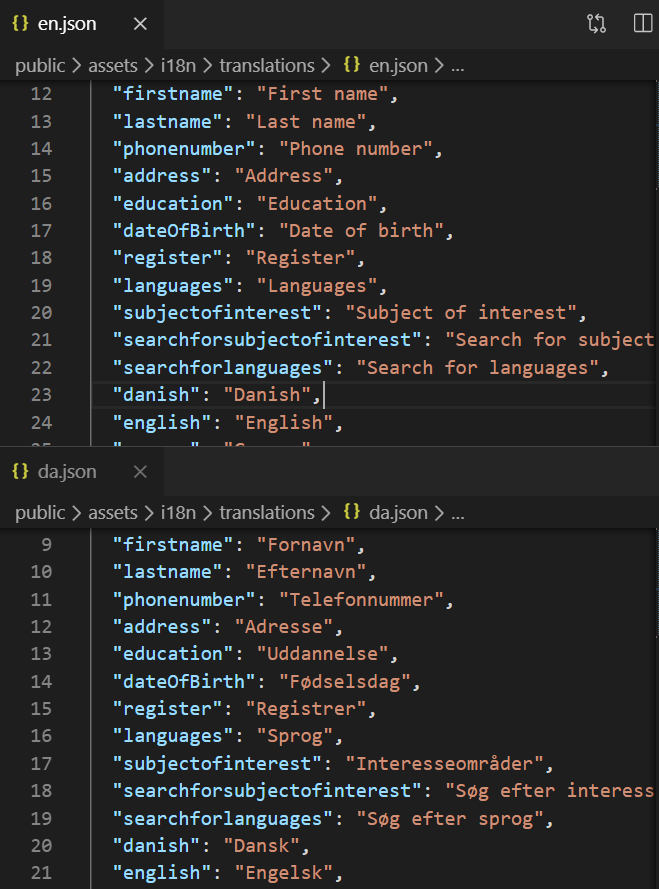
\includegraphics[scale=0.5]{figures/translations.PNG}
    \caption{The Danish and English translation files}
    \label{fig:translationfiles}
\end{figure}
\noindent
To add an additional language all that needs to be done is to make a new file and translate all the lines. 
It is not necessary to refactor any code to add additional languages.